\documentclass[12pt]{article}

\usepackage{sbc-template}

\usepackage{graphicx,url}

\usepackage{amssymb}
\usepackage{amsmath}

\usepackage{float}
\usepackage[utf8]{inputenc}  

     
\sloppy

\title{(Algo nesse sentido) Utilização de transitividade e simetria para geração de dados}

\author{Alison Sassi\inst{1}, Gustavo Spiess\inst{2} }

\address{Departamento de Ciências Exatas e Engenharias\\
Universidade Regional do Noroeste do Estado do Rio Grande do Sul
  (UNIJUÍ)\\
  Rua do Comércio, 3000, Universitário -- 98700-000 -- Ijuí -- RS -- Brazil
  \email{\{alisonsassij,gspiess\}@gmail.com}
}

\begin{document} 

\maketitle

\section{RESUMO}

Nos últimos cem anos, a maior pandemia ocasionado pela doença da COVID19 em 2020 foi a mais mortal, presenciamos um cenário do colapso da estrutura hospitalar pública, falta de leitos, falta de respiradores e também profissionais da saúde. Os leitos de Unidade de Terapia Intensiva (UTI) foram alocados na sua totalidade, nesse momento os médicos tiveram um enorme desafio de entender a prioridade de um paciente em um leito de UTI, ocasionando em problemas psicológicos, muitas vezes sendo uma escolha baseado no emocional do médico . Durante esse período, médicos realizaram uma decisão de quem ocupava um leito disponível, utilizando protocolos de triagem e guias criados por vários lugares do mundo, para minimizar a quantidade de mortes.

Em um cenário onde as internações de pessoas em leitos de Unidade de Terapia Intensiva (UTI) aumentaram gradativamente diante dos casos clínicos críticos suscitados pelo vírus causador da COVID-19 ocasionando a escassez de leitos hospitalares, o médico intensivista vivenciou a inquietude de uma decisão da escolha do próximo paciente a medida que os leitos vão sendo desocupados, ocasionando problemas psicológicos, muitas vezes sendo uma escolha baseado no emocional do médico. Neste cenário as decisões equivocadas podem ocasionar o mau uso de leitos de UTI com processos de distanásia contribuindo  ainda mais, para escassez de leitos. Com um modelo computacional capturando as variáveis de decisão baseada em dados do paciente, o profissional poderá se apoiar na transparência da sugestão que o modelo oferecerá. Para esse modelo baseado em dados do paciente se tornar algo factível, será necessário utilizar um protocolo que através de variáveis informadas, possa fazer uma listagem dos pacientes que necessitarão de um leito de UTI. Este artigo tem por objetivo descrever o modelo utilizado para a triagem, explica a forma que as variáveis foram extraídas e demonstra a criação da geração de uma base de dados para uma validação dos dados com médicos especialistas.

\textbf{Palavras-chave:} Unidade de Terapia Intensiva (UTI). Escassez de leitos hospitalares. Auxílio médico. Gerenciamento hospitalar. Protocolo.

\section{ABSTRACT} 
In a scenario where admissions in Intensive Care Unit (ICU) beds gradually increased due to critical clinical cases caused by the COVID-19 virus, resulting in a shortage of hospital beds, the intensivist physician experienced the anxiety of deciding on the next patient as the beds are being vacated, causing psychological problems, often being a choice based on the physician's emotions. In this scenario, wrong decisions may cause misuse of ICU beds with dysthanasia processes, contributing even more to the shortage of beds. With a computer model capturing the decision variables based on patient data, the professional will be able to rely on the transparency of the suggestion that the model will offer. For this model based on patient data to become feasible, it will be necessary to use a protocol that through informed variables, can list the patients who will need an ICU bed. This article presents the model used, the way the variables were treated and the generation of a database for validation with medical specialists.

\textbf{Keywords:} Intensive Care Unit (ICU). Shortage of hospital beds. Medical assistance. Hospital management. Protocol.

\section{INTRODUÇÃO}
% A oferta de leitos de Unidade de Terapia Intensiva (UTI) é historicamente escassa no Brasil \cite{murthy2015intensive}. Em 2018 o Conselho Federal de Medicina (CFM) realizou uma pesquisa tendo como base a indicação da Associação de Medicina Intensiva Brasileira na qual se aponta a necessidade de 1 a 3 leitos de UTI para cada 10 mil habitantes \cite{domingues2018numero}. De acordo com o Conselho Federal de Medicina, no ano de 2018, 21.500 leitos de UTI no Brasil foram disponibilizados pelo Sistema Único de Saúde (SUS) \cite{cfm2018,cfm2020}.
Conforme o Conselho Federal de Medicina, em fevereiro de 2020 o Cadastro Nacional de Estabelecimentos de Saúde indicava a existência de 46 mil unidades de UTI, sendo metade disponível para o SUS e a outra metade reservada aos planos de saúde e à rede privada. Ao longo de 10 anos, entre junho de 2011 e junho de 2020, esse número aumentou em torno de 38\%. Com o surgimento da pandemia do covid-19, de fevereiro a junho de 2020 o número de leitos no SUS aumentou cerca de dez mil unidades totalizando 31.800 leitos de UTI no Brasil.
De acordo com \textbf{Pitta (2021)}, mesmo com o aumento de leitos, ainda há apenas uma unidade de terapia intensiva para aproximadamente dez mil habitantes no Brasil, o que debilita o sistema público de saúde e o deixa extremamente frágil para enfrentar situações pandêmicas, como a que vivemos atualmente \cite{pimentel2020design}. Durante a pandemia, foi necessário aumentar drasticamente o número de leitos no Brasil em cerca de 45\% no primeiro semestre de 2020, mas segundo \textbf{CFM (2020)}, os órgãos federais estão solicitando devoluções de leitos, o que reduzirá drasticamente o número de leitos no período pós pandemia.
% Historicamente o Brasil tem uma carência de leitos disponíveis para a população, a pandemia trouxe uma superlotação de leitos e sobrecarga dos profissionais. Em São Paulo, Estado que tem a maior estrutura hospitalar do país, no primeiro trimestre de 2021, morreram pelo menos 135 pessoas à espera de uma vaga na UTI. O Paraná, no mesmo período, totalizou 500 mortes aguardando a disponibilidade de leitos de UTI e enfermaria, e 1.196 paranaenses aguardavam por uma vaga, segundo o governo do Estado \cite{fundacaooswaldocruz2021}. Além da falta de vagas, faltam médicos capacitados para trabalhar nas unidades; Segundo \textbf{Martins (2021)} “O ideal seria que o país tivesse cinco a seis vezes mais a quantidade de médicos intensivistas do que temos hoje para atender com plena capacidade em todos os leitos de UTI”.
% Uma pesquisa realizada pela Fundação Getúlio Vargas e Fundação Oswaldo Cruz consultou 1.829 profissionais de saúde no Brasil em março de 2021, 85,4\% dos médicos entrevistados relataram que tiveram sua saúde mental afetada negativamente pela pandemia \cite{paulomotoryn2021}. Um dos pontos que influenciam diretamente e tem provocado grandes mudanças psicológicas negativas durante a pandemia, é a responsabilidade que o médico tem de escolher qual paciente tem o quadro clínico mais adequado para poder ocupar um leito de UTI \cite{teixeira2020processo}.
% Diante da complexidade e inusitados casos clínicos, a tomada de decisão exige mais rapidez, assertividade na resposta e baseado nos dados pessoais do paciente, agilizando o processo de ocupação do leito de UTI e também para outros pacientes que estão na espera. Alguns trabalhos estão desenvolvendo plataformas para trocas de informações interprofissionais entre as áreas médicas \cite{santos2020desenvolvimento}. Outros estão preocupados em encontrar uma forma de otimizar os leitos de UTI \cite{pinto2019alocaccao} utilizando variáveis comuns entre os pacientes para a alocação dos leitos de UTI. Muitos destes estudos não levam em consideração a personalização dos dados pessoais do paciente, realizando uma programação que pode ser equivocada dependendo do caso clínico.
Com um modelo computacional capturando as variáveis de decisão baseada em dados do paciente, o profissional poderá se apoiar na transparência da sugestão que o modelo oferecerá. Para esse modelo baseado em dados do paciente se tornar algo factível, será necessário utilizar um protocolo que através de variáveis informadas, possa fazer uma listagem dos pacientes que necessitarão de um leito de UTI. O sistema utilizará modelo de Inteligência Artificial(IA), supervisionado, treinado para que o médico visualize os dados do paciente e sua respectiva prioridade dentre os que necessitam de internação na UTI.


\section{MÉTODO CIENTÍFICO}

% Trata-se de uma pesquisa exploratória/explicativa, que visa propagar para os pesquisadores a identificação do problema e na proposição de uma solução computacional para analisar dados e indicar pacientes, conforme o Protocolo AMIB de alocação de recursos em esgotamento durante a pandemia por COVID-19 escolhido \cite{kretzer2020protocolo}.
% Inicialmente foi realizada uma pesquisa bibliográfica, a partir da qual os pesquisadores buscaram conhecer a área em questão, identificando as melhores alternativas de solução. Em seguida, a pesquisa se tornará experimental, a fim de obter os resultados em um software contendo o modelo e a estrutura necessária para seguir na homologação, com dados que serão inseridos. 
% Para apresentar a solução de maneira científica, deve ser escolhida uma metodologia que coincide com o objetivo da pesquisa. Design Science Research, é um método científico que trabalha com artefatos informacionais eficientes, tendo hipóteses teóricas fundamentadas no estado da arte e da técnica, resultando em produção do conhecimento científico pelo rigor do processo \cite{pimentel2020design}.
% Nos resultados a seguir, está explicada a fase técnica para geração dos dados que serão homologados na fase de validação do modelo computacional da pesquisa.

\section{PROPOSTA DA PESQUISA}
No cenário em que o setor de UTI em um hospital está com todos os leitos ocupados, e ainda, pacientes esperando por uma vaga, o médico encarregado deve definir qual paciente será o próximo a ocupar um leito da UTI quando estiver vago. Amiudadamente o médico elege o paciente, com condições físicas e/ou emocionais como, uma alta carga de estresse, constante tensão emocional baseado em sentimentos e cansaço físico, que podem influenciar na decisão.
Conhecendo esses problemas, tem-se buscado a tecnologia para auxiliar o profissional de saúde a diminuir a grande carga que possui. Uma solução que se encaixa para resolver esse problema, é a inteligência artificial (IA), com ela é possível ensinar o sistema para fazer um posicionamento através de variáveis bem definidas em um modelo computacional criado, onde deve estar diretamente conectado nos dados de saúde de cada paciente.
% Os critérios que o modelo computacional utilizará, estão baseados em um protocolo utilizado pelos profissionais de saúde, portanto, para essa solução, foi escolhido como base o protocolo publicado em 2020 pela Associação de Medicina Intensiva Brasileira (AMIB), fundamentado no modelo do protocolo de triagem proposto por \textbf{Biddison et al.}\cite{biddison2019too} e se assemelha ao modelo do protocolo de triagem proposto por \textbf{White}\cite{white2009should, white2020}.
A proposta deste projeto tem a intenção de disponibilizar ao médico uma listagem dos pacientes promovendo o acesso transparente a leitos de UTI escassos. Possibilitará uma alta velocidade na decisão, com o uso da inteligência artificial, entregará uma assertividade baseada em dados do paciente e nas recomendações da Associação de Medicina Intensiva Brasileira (AMIB) para a abordagem do covid-19.


\section{ARQUITETURA}
A proposta da arquitetura tem objetivo de otimizar tempo neste trabalho, pois se baseará no framework django, composta com a arquitetura MTV (Model, Template, View). A camada Template é a responsável pelas páginas visuais, onde o usuário estará em contato direto, enviando as informações para a próxima camada. A camada View recebe as informações que estão sendo enviadas e as processa conforme a programação, devolvendo as informações para o Template. A View é uma camada intermediária da arquitetura, tendo contato contínuo com a camada Model. Por fim, a camada Model tem a responsabilidade de conexão entre o sistema gerenciador de banco de dados, PostgreSQL, com a camada View.
Na Figura abaixo é demonstrado de forma abrangente, como as camadas da arquitetura se conectam para chegar no resultado final. Existe a interface que está diretamente conectada com o médico, sendo uma interação humano-computador. A partir desta camada, é realizada a comunicação com a regra de negócio definida no sistema e o modelo computacional. Após o processamento das informações, o resultado esperado será retornado na interface para o médico, a listagem realizada.

\begin{figure}[!htb]
    \centering
    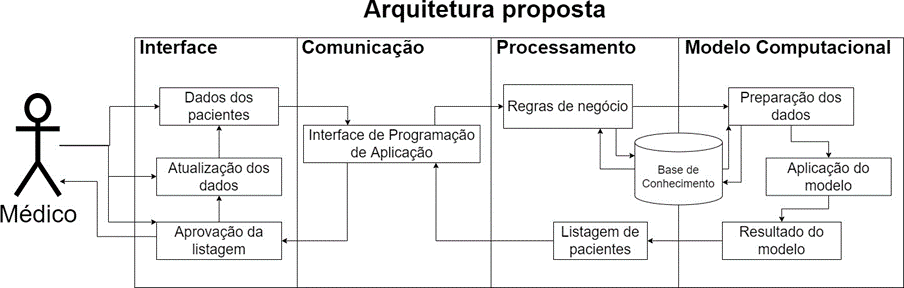
\includegraphics[scale=0.9]{img/Arquitetura-MDS.png}
    \centering
    \caption{Arquitetura proposta para a pesquisa.}
    \label{subexpressao1}
\end{figure}

Somente a arquitetura não é capaz de criar o sistema, deve existir tecnologias para a implementação das regras e modelo, assim como a estilização e funcionalidades da interface. Para isso propõem-se utilizar algumas tecnologias que são fundamentais para criação do sistema, tais como: HyperText Markup Language (HTML), para construção de páginas na Web; Cascading Style Sheets (CSS), para estilização das páginas; e a linguagem de programação JavaScript, para ações nas páginas, gerando a interface do sistema.

\section{MODELO COMPUTACIONAL}

Considerando o protocolo AMIB, existem nove critérios clinicos a serem havaliados para a tomada de decisão, denotados $a_1$ até $a_9$:

\[
    \begin{split}
        a_1 &\in \mathbb{Z}; 20 \ge a_1 \ge 85\text{, sendo a idade do paciente} \\
        a_2 &\in \{0, 1, 2, 3, 4\}\text{, sendo o critério neurológico} \\
        a_3 &\in \{0, 1, 2, 3, 4\}\text{, sendo o critério respiratório} \\
        a_4 &\in \{0, 1, 2, 3, 4\}\text{, sendo o critério cardio-vascular} \\
        a_5 &\in \{0, 1, 2, 3, 4\}\text{, sendo o critério renal} \\
        a_6 &\in \{0, 1, 2, 3, 4\}\text{, sendo o critério hepático} \\
        a_7 &\in \{0, 1, 2, 3, 4\}\text{, sendo o critério eu não lembro mais} \\
        a_8 &\in \{0, 3\}; a_1 < 60 \implies a_8=0\text{, sendo o critério oncológico} \\
        a_9 &\in \{0, 1, 2, 3, 4\}\text{, sendo o critério de comorbidades} \\
    \end{split}
\] 

Notadamente, o protocolo não limita a idade para apneas as faixas descritas, o procolo é aplicável para situações conde há pacientes com menos de vinte anos ou com mais de oitenta e cinco.
Essa restrição de idade foi decidida em prol da geração de dados, e poderia ser modificada.
Outra observação que de deve ressaltar é de que o critério oncológico é sujeito, no protocolo AMIB, à idade do paciente, isso é, mesmo com indicação clínica de tumores, o critério só os considera para pacientes com mais de sessenta anos.

Para a execução do protocolo são utilizadas as seguintes somas:

\[
\begin{split}
    s &= \sum_{n=2}^{7} a_n\text{, sendo o SOFA} \\
    t_1 &=  \begin{cases}
        0, \text{se } a_1 < 99 \\
        1, \text{se } 99 < a_1 < 99 \\
        2, \text{se } 99 < a_1 < 99 \\
        3, \text{se } 99 < a_1 < 99 \\
        4, \text{se } 99 < a_1 \\
    \end{cases} \\
    t_2 &= \begin{cases}
        0, \text{se } s < 99 \\
        1, \text{se } 99 < s < 99 \\
        2, \text{se } 99 < s < 99 \\
        3, \text{se } 99 < s < 99 \\
        4, \text{se } 99 < s \\
    \end{cases} \\
    t &= t_1 + t_2 + a_8 + a_9 \\ % TODO revisar a soma
\end{split}
\] 

Dados dois pacietnes, $p_1$ e $p_2$, o protocolo decide entre os dois primeiramente comparando o valor de $t$ calculado para cada um, se  $t_{p_1}$ for menor que $t_{p_2}$ o protocolo prescreve que a preferência na obtenção do leito seja de  $p_1.$
A reciproca, naturalmente, é verdadeira.
No caso de $t$ ser igual para os dois pacientes, é realizada a comparação usando  $s$. 
No caso de $t$ e de  $s$ serem iguais para os pacientes, utiliza-se o EU JÁ NEM ME LEMBRO MAIS.

Notadamente, é possível desenhar dois pacientes para que o protocolo seja incapaz de fornecer distinção relevante a respeito de priorização de um em relação a outro, no caso em que o protocolo sugere randomização.
Mais especificamente, é possível desenhar uma função $\alpha \in [0, 1]$ que informe o grau de certeza com o qual o protocolo determina a prioridade.

\[
\alpha = \begin{cases}
    \frac{t_{p_1} - t{p_2}}{\max_t - \min_t}, \text{se } t_{p_1} - t_{p_2} \neq 0 \\
    \frac{s_{p_1} - s{p_2}}{\max_s - \min_s}, \text{se } s_{p_1} - s_{p_2} \neq 0 \\
    \ldots \\
    0, \text{se o protocolo prescreve randomização}
\end{cases}
\] 

Sendo um objetivo minimizar $\alpha$, é preciso destavar de que isso é trivial considerando o caso de dois pacientes com todos os critérios idênticos, mas esse caso foge do que é desejável, pois não são cabíveis quaisquer outros argumentos quanto a priorização.
Para tando, se utiliza-se a noção de inercia ($i$) como medida de homogeneitdade, de forma que valores menores de $i$ implicam conjuntos de paciêntes mais homogêneos.
A inércia pode ser calculada como o quadrado da disância de cada menbro do conjunto para o centro de gravidade do conjunto.

\[
i = \sum_{p \in P}d(p, c)^2
\] 

Considerando $P$ o conjunto de pacientes, $c$ o centro de massa desse conjutno e $d$ a distância euclideana.

Com essas definições, é possível a construção de um conjunto de dados que maximize a obtenção de quais os critérios de decisão de um médico, presumindo que ele se informe pelo protocolo AMIB, mas que tome uma decisão médica para os casos em que o trotocolo prescreve randomização.
Para tanto, qualquer que seja o conjunto de pacientes que o médico ordenará, esse deve maximizar a inercia e minimizar alfa.

Considerando uma função de qualidade $\frac{i}{\alpha}$, razliza-se uma busca por um conjunto de dez pacientes da seguintes forma:

\section{ETAPA DE VALIDAÇÃO}
O processo de validação proposto, é através de casos clínicos hipotéticos, elaborados por grupos de médicos com experiência na área do setor de UTI que reflitam a realidade cotidiana. Os casos deverão ser cadastrados previamente na solução e validados por um profissional da saúde. Cada caso cadastrado na base será alocado a um grupo divididos em dez registros de pacientes, podendo se repetir nos grupos, conforme a aleatoriedade de um algoritmo para que não haja influência humana.
Um ou mais grupos de pacientes  terá  um  médico  que  fará  a  listagem  ordenada por prioridade, posteriormente comparado o resultado da listagem que o modelo elegeu, finalizando com um consenso entre ambas listagens, definindo se o modelo deve ter mais um ciclo de aprendizagem.
A proposta para a validação é possuir dez médicos voluntários para participar, avaliando os casos clínicos hipotéticos, realizando a separação entre os grupos de pacientes.
Os médicos voluntários terão em mãos os dados sintéticos de pacientes, com possibilidade de visualizar com detalhes cada dado clínico, realizando a escolha da posição da listagem dos pacientes. Após a escolha o médico terá o resultado do modelo desenvolvido e por fim será realizado uma entrevista para entender a divergência de opinião com o consenso entre as listagens.

\section{RESULTADOS}

Até o momento, foram realizadas a extração dos dados do Protocolo AMIB de alocação de recursos em esgotamento durante a pandemia por COVID-19, publicação do ano de 2020, as quais foram selecionadas 9 variáveis clínicas de pacientes:
1.	Idade do paciente, variável extraída do protocolo AMIB 2020.
2.	Sintomas neurológicos, variável extraída do protocolo SOFA.
3.	Sintomas cardiovasculares, variável extraída do protocolo SOFA.
4.	Sintomas respiratórios, variável extraída do protocolo SOFA.
5.	Exames de coagulação, variável extraída do protocolo SOFA.
6.	Sintomas hepáticos, variável extraída do protocolo SOFA.
7.	Sintomas renais, variável extraída do protocolo SOFA.
8.	Avaliação do Índice de Comorbidade de Charlson (ICC), variável extraída do protocolo AMIB 2020.
9.	Avaliação da escala Performance Status do Eastern Cooperative Oncology Group (ECOG), variável extraída do protocolo AMIB 2020.
Para propor o algoritmo de aprendizado de máquina supervisionado capaz de interpretar os critérios, é necessário ter uma quantidade de dados já avaliados por especialistas. Anteriormente à etapa aprendizado de máquina, utilizou-se a linguagem de programação propósito geral, muito utilizada em atividades de análise de dados (LOPES, 2019) para gerar uma massa de dados planejada e preparada para a validação.
O pacote Faker desenvolvido para a linguagem Python, que gera nomes reais anonimizados pelo algoritmo de forma mesclada, proporcionou uma geração da massa de dados de forma simples, e eficaz, assim como o pacote Random que gera números pseudo-aleatórios conforme necessidade. Ambos utilizados para gerar uma massa de dados predefinida pelo protocolo AMIB de 2020.
Com as 6 variáveis do SOFA sendo geradas entre números inteiros entre 0 e 4, a variável ICC gerada somente nos números 2 ou 4 e por fim a variável ECOG sendo gerada entre os números 0 e 4 para pacientes que tiverem mais de 60 anos. Desta forma, a uma massa de dados gerada foi armazenada como mostra no segmento de dados abaixo:

\begin{figure}[!htb]
    \centering
    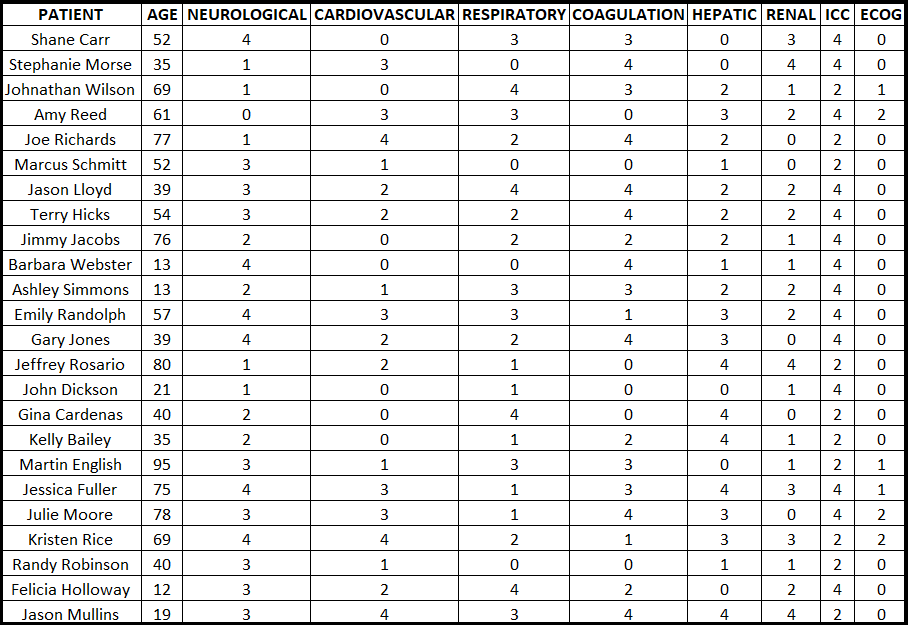
\includegraphics[scale=0.6]{img/massa de dados gerada.png}
    \centering
    \caption{Massa de dados gerada.}
    \label{subexpressao2}
\end{figure}

O modelo proposto no protocolo AMIB 2020 foi composto por um sistema de avaliação de múltiplos critérios que representam diferentes objetivos éticos: i) salvar o maior número de vidas; ii) salvar o maior número de anos/vida; iii) equalizar as oportunidades de se passar pelos diferentes ciclos da vida. O sistema de pontuação pode variar do número dois a onze, onde quanto menor é a pontuação de um paciente, maior será a sua prioridade de alocação de recursos escassos. Quanto maior o número de pacientes a serem triados, maior será a expectativa de empates nas pontuações e por esta razão o protocolo, assim como o de Biddinson et al, também inclui sugestões de critérios de desempate, os quais serão calculados juntos com a base de treinamento, para isso levantou-se os critérios. Em caso de desempate o presente modelo sugere os seguintes critérios de desempate sequenciais:
\begin{itemize}
  \item Escore de fragilidade clínica;
  \item Pontuação total do SOFA;
  \item Randomização.
\end{itemize}

Um segmento da base de dados gerado sinteticamente, o qual contém o cálculo de critérios de desempate, será utilizado para que a Rede Neural possa analisar em conjunto com os dados de cada paciente.

\begin{figure}[!htb]
    \centering
    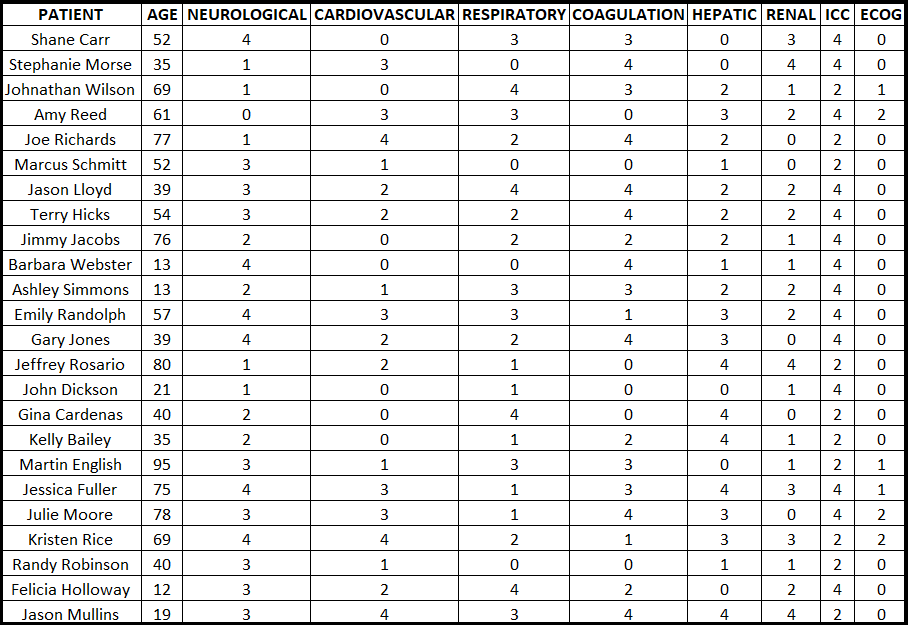
\includegraphics[scale=0.6]{img/massa de dados gerada.png}
    \centering
    \caption{Massa de dados gerada com critérios.}
    \label{subexpressao}
\end{figure}

Com os dados gerados, foi possível criar um sistema capaz de separar em grupos definidos de dez registros, distribuídos de forma agrupada com o objetivo de que uma equipe médica possa validar a ordenação de cada grupo, entendendo qual paciente deve ter a prioridade conforme sua experiência. 
Um ou mais grupos serão compostos por dez registros hipotéticos, com as variáveis extraídas do protocolo AMIB de alocação de recursos em esgotamento durante a pandemia por COVID-19, sendo validados com um médico especialista de forma de listagem em ordem de prioridade conforme sua experiência profissional.
Será utilizada a mesma base de dados com as avaliações médicas, inserindo os dados no modelo computacional para ensinar um algoritmo de inteligência artificial a realizar uma listagem dos pacientes que estão na espera de um leito de UTI.

\section{PRÓXIMAS ETAPAS}
Após esse resultado mapeado e esperado, as próximas etapas para o desenvolvimento da aplicação proposta no projeto é propor e escrever o algoritmo de aprendizado de máquina supervisionado capaz de interpretar os critérios, realizar a validação do modelo, treinar o algoritmo com os dados dos critérios extraídos, realizar e qualificar a validação do modelo construído, reajustando se necessário.
E por fim a validação dos dados gerados com o grupo de médicos voluntários o qual será realizado por especialistas que possam validar o modelo e ensinar a rede neural com a experiência de médicos.

\section{CONSIDERAÇÕES FINAIS}
No presente trabalho tratou-se do problema de pesquisa identificado sobre a escassez de leitos de unidade de terapia intensiva, levantando uma solução para o auxílio do médico intensivista.
Foi descrito as etapas técnicas para geração de uma base de dados conforme planejamento da pesquisa que está em andamento, como também a forma de validação destes dados.
O sistema auxiliará o médico intensivista em um hospital quando os leitos de UTI estiverem escassos, utilizando um modelo computacional para geração de uma lista de pacientes.

\section{REFERÊNCIAS BIBLIOGRÁFICAS}

\bibliographystyle{sbc}
\bibliography{sbc-template}

\end{document}

